Below we depict additional results for the airline data set using a hypothesis space of LIN, PER, SE and RQ covariance functions as base kernels for the composition. Fig \ref{fig:airline1} shows the training data and posterior samples drawn from the \ac{GP} with posterior composite structure. 

\begin{figure}
\includegraphics[width=\textwidth]{figs/posterior_samples_airline.png}
\caption{Data (black x) and posterior samples (red) for the airline data set.}\label{fig:airline1}
\end{figure}
Fig. \ref{fig:posterior_twosamples} shows why it advantageous to be Bayesian here. We see two possible hypotheses for the composite structure of $\mathbf{K}$. 

\begin{figure}
        \centering
        \begin{subfigure}{0.49\textwidth} \centering
                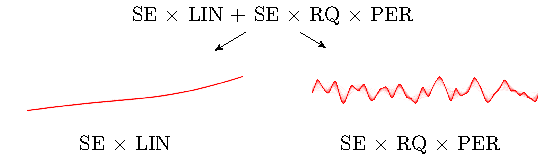
\includegraphics[width=0.9\textwidth]{figs/airline_struct_1.pdf}
        \end{subfigure}
	\begin{subfigure}{0.49\textwidth} \centering
                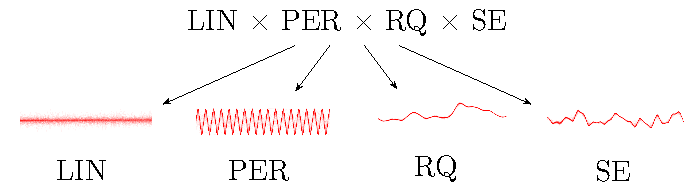
\includegraphics[width=0.8\textwidth]{figs/airline_struct_2.pdf}
        \end{subfigure}
        \caption{We see two possible hypotheses for the composite structure of $\mathbf{K}$. (a) Most frequent sample drawn from the posterior on structure. We have found two global components. First, a smooth trend (LIN $\times$ SE) with a non-linear increasing slope. Second, a periodic component with increasing variation and noise. (b) Second most frequent sample drawn from the posterior on structure. We found one global component. It is comprised of local changes that are periodic and with changing variation.}\label{fig:posterior_twosamples}
\end{figure}